\chapter{Analyse spectrale paramétrique}
\noindent L'objectif global de ce domaine est de récupérer les informations sur le signal $X$ à partir de $N$ observations, tel que :
    \[ X =
    \begin{bmatrix}
        x(1) & x(2) & ... & x(N)
    \end{bmatrix}
    \]
\noindent On considère alors que le signal $X$ appartient à une famille de signaux qui dépendent d'un paramètre $\theta$ en utilisant une méthode paramétrique \footnote{paramétrique, Bayésien : Le paramètre $\theta$ est supposé aléatoire de loi cconnue}.
Les méthodes paramétriques permettent de d'obtenir des informations sur le signal tels que les raies et l'enveloppe spectrale. Le but est, par la suite, d'interpréter ces résultats.
\begin{figure}[hbt!]
    \centering
    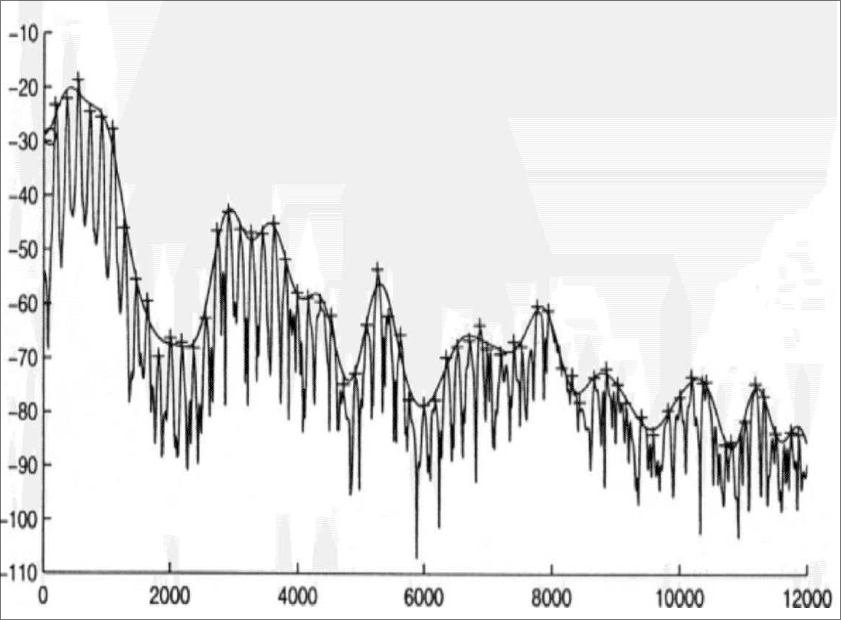
\includegraphics[scale=0.5]{Pics/Enveloppe.png}
    \caption{Enveloppe spectrale d'un signal $X$}
\end{figure}
\newpage
\section{Incertitude de Gabor}
\noindent De même que pour le principe d'incertitude d'Heisenberg, l'analyse spectrale comporte des incertitudes. En effet, les signaux analysés/observés sont stationnaires ou pseudo-stationnaires sur de courtes périodes, ce qui contraint l'étude des signaux pour des périodes de l'ordre de $\Delta T = 40ms$. \newline

\noindent De ce fait, on appelle $\Delta f$ la \textbf{distance en fréquences entre deux raies}, et on introduit le principe d'incertitude de Gabor tel que :
\begin{equation}
    \normalsize
    \tcbhighmath[fuzzy halo=0.5mm with electricultramarine!35!electricultramarine,arc=2pt,
    boxrule=0pt,frame hidden]{ 
        \Delta f \Delta T = cste
    } \nonumber
    \normalsize
\end{equation}
Les méthodes dites \textit{hautes résolutions}\footnote{donc avec une $\Delta T$ grand} ont une perte d'informations trop grande, ce qui perd un peu l'intérêt de l'analyse spectrale. En revanche, on peu utiliser des méthodes de haute résolution en considérant la fonction \textbf{coût} qui dépend des amplitudes des raies $a_{i}$ et de leurs déphasages $\phi_{i}$. 
\section{Modèles auto-régressifs}
\subsection{Modèle ARMA}
Modélisation des signaux $x_{n} = x[n]$ :
\begin{equation}
    \normalsize
    \tcbhighmath[fuzzy halo=0.5mm with electricultramarine!35!electricultramarine,arc=2pt,
    boxrule=0pt,frame hidden]{ 
        x_{n} = x[n] = \sum_{i=0}^{q}{b_{i}n_{n-i}} - \sum_{i=0}^{p}{a_{k}n_{n-k}}
    }
    \normalsize
\end{equation}
Avec :
\begin{itemize}
    \item $x_{n}$ : signal à modéliser
    \item $a_{k}$ et $b_{i}$ : estimateurs (paramètres) à déterminer
    \item $n_{n} = n_[n]$ : bruit blanc gaussien \newline
\end{itemize}
\noindent Ce modèle est relativement difficile à exploiter, notament à cause des $b_{i}$
\subsection{Modèle AR - AR, auto-régressifs}
On reprend le modèle ARMA et on pose $q=0$ et $b_{0}=1$, soit : 
\begin{equation}
    \normalsize
    \tcbhighmath[fuzzy halo=0.5mm with electricultramarine!35!electricultramarine,arc=2pt,
    boxrule=0pt,frame hidden]{ 
        x_{n} = x[n] = n_{n} - \sum_{k=0}^{p}{a_{k}n_{n-k}}
    }
    \normalsize
\end{equation}
\textbf{Objectif : estimer les $a_{k}$ en minimisant la variance $\sigma^{2}$ du bruit $n$} \newline
\noindent Pour se faire, il existe plusieurs algorithmes, tels que :
\begin{itemize}
    \item Levinson-Durbin (ou Yule-Walker)(faisable)
    \item Burg (faisable)
    \item Marple (assez difficile)
\end{itemize}
\newpage
\subsection{Levinson-Durbin - Yule-Walker}
Il faut d'abord estimer les \textbf{coefficients d'autocorrélation} $\widehat{R}_{xx}$ du signal $x \in \mathbb{K}^{n}$ 
\Large
\begin{align}
    \widehat{R}_{xx}[k] &= E[x_{n+k}x^{*}_{n}] \nonumber\\
                        &= E[x^{*}_{n}(-\sum_{i=0}^{p}{a_{i}n_{n-i+k} + n_{n+k}})] \nonumber \\
    \widehat{R}_{xx}[k] &=-\sum_{i=1}^{p}{a_{i}\widehat{R}_{xx}(-i+k) + E[n_{n+k}x^{*}_{n}]} \nonumber
\end{align}
\normalsize
\subsubsection{Fonction de transfert}
Pour ce filtre stable, linéaire et causal : 
\begin{equation}
    H(z) = \frac{1}{A(z)} = \frac{1}{\sum_{m=0}^{p}{a_{m}z^{-m}}}
\end{equation}
Avec $a_{0} = 1$. On obtient alors les 
\subsubsection{Equations de Yule-Walker}
\Large
\begin{equation}
    R_{xx}[k] = -\sum_{i=1}^{p}a_{i}\widehat{R}_{xx}[k-i], k \in {\mathbb{R}^{*}}^{+}
\end{equation}
\begin{equation}
    R_{xx}[k] = -\sum_{i=1}^{p}a_{i}\widehat{R}_{xx}[k-i] + \sigma^{}, k = 0
\end{equation}
\normalsize
\newpage
\noindent Ce qui donne en écriture matricielle :
\Large
\[
\begin{bmatrix}
    R_{xx}[0] & R_{xx}[-1] & \dots & R_{xx}[-(p-1)] \\
    R_{xx}[1] & R_{xx}[0]  & \dots & R_{xx}[-(p-2))] \\
    \vdots    & \vdots     & \ldots& \vdots \\ 
    R_{xx}[p-1] & R_{xx}[p-2] & \dots & R_{xx}[0)]
\end{bmatrix}
\begin{bmatrix}
    a_{1} \\
    a_{2} \\
    \vdots \\
    a_{p}
\end{bmatrix}
=
\begin{bmatrix}
    R_{xx}[1] \\
    R_{xx}[2] \\
    \vdots \\
    R_{xx}[p]
\end{bmatrix}
\]
\normalsize
ou bien :
\Large
\[
\begin{bmatrix}
    R_{xx}[0] & R_{xx}[-1] & \dots & R_{xx}[-p] \\
    R_{xx}[1] & R_{xx}[0]  & \dots & R_{xx}[-(p-1))] \\
    \vdots    & \vdots     & \ldots& \vdots \\ 
    R_{xx}[p-1] & R_{xx}[p-2] & \dots & R_{xx}[0)]
\end{bmatrix}
\begin{bmatrix}
    1 \\
    a_{2} \\
    \vdots \\
    a_{p}
\end{bmatrix}
=
\begin{bmatrix}
    \sigma^{2} \\
    0 \\
    \vdots \\
    0
\end{bmatrix}
\]
\normalsize
Ces matrices donnent accès aux $(a_{i})_{i \in \mathbb{N}}$